\newpage
\section{Object Oriented Programming}
\subsection{Modularità}
La \textbf{modularizzazione} è una tecnica utilizzata nella programmazione per sviluppare un programma per livelli di astrazione. Ad esempio:
\begin{itemize}
	\item Sotto il profilo \textbf{linguistico} c'è l'astrazione procedurale, che permette di scomporre il problema in sottoproblemi
	\item Sotto il profilo dei \textbf{tipi di dato} abbiamo i tipi di dato astratti
	\item Sotto il profilo delle \textbf{tecniche di compilazione} troviamo la compilazione separata ed il linking
\end{itemize}
La combinazione di \textbf{astrazione} e \textbf{problem solving} consentono di trovare soluzioni efficienti a problemi complessi.\\
Nell'ambito dell'\textit{ingegneria del software} la modularità permette di suddividere il lavoro tra sviluppatori diversi:
\begin{itemize}
	\item Si definiscono le \textbf{specifiche} delle diverse parti (anche grazie ai diagrammi UML)
	\item Ognuno sviluppa la sua
\end{itemize}

\subsection{Oggetti}
Un software, nell'ambito della OOP, è un insieme di oggetti cooperanti, dove ogni oggetto è caratterizzato da:
\begin{itemize}
	\item Uno \textbf{stato}
	\item Un insieme di \textbf{funzionalità}
	\item Un'\textbf{identità}, ovvero il nome che individua l'oggetto
	\item Il \textbf{ciclo di vita}, quindi la creazione, il riferimento e la disattivazione
	\item La \textbf{locazione} di memoria
\end{itemize}
I vari oggetti comunicano tra di loro scambiandosi messaggi.
\subsubsection{Stato}
Lo stato di un oggetto è rappresentato da un grupopo di attributi. Deve rispettare la proprietà di \textbf{incapsulamento}:
\begin{definition}[Incapsulamento]
	Lo stato di un oggetto non dovrebbe essere accessibile dagli altri oggetti. Bisogna fare \textbf{information hiding}.
\end{definition}
Lo stato di un programma è invece l'insieme degli stati degli oggetti che lo compongono.
\subsubsection{Funzionalità}
Le funzionalità di un oggetto sono rappresentate da un gruppo di \textbf{metodi} che l'oggetto mette a disposizione degli altri oggetti. Questi descrivono il comportamento dell'ggetto, ovver come questo risponde ad un messaggio ricevuto (modificando il proprio stato o interagendo con altri oggetti). Solitamente:
\begin{itemize}
	\item L'\textbf{invio} di un messaggio corrisponde ad una chiamata di metodo
	\item La \textbf{risposta} di un messaggio corrisponde alla restituzione del risultato
\end{itemize}

\subsection{Strutture linguistiche}
I linguaggi di programmazione supportano l'OOP seguendo due approcci principali:
\begin{itemize}
	\item \textbf{Object-based}, come JS, Self, Lua
	\item \textbf{Class-based}, come C++,Java,Scala
\end{itemize}
\subsubsection{Object-based}
In questo approccio gli oggetti vengono trattati come \textbf{record}. I campi possono essere associati a funzioni (\textbf{metodi}) e questi possono accedere ai campi stessi tramite il riferimento \textit{this}. In alcuni casi è anche possibile \textbf{modificare} la struttura dell'oggetto dinamicamente.
\begin{example}[JS Object-based]
	\begin{lstlisting}
		let mario = {
			nome: "Mario",
			cognome: "Rossi",
			eta: 35,
			compleanno: function() {
				this.eta += 1;
			}
		}
		
		console.log(mario.nome); // Mario
		console.log(mario.eta); // 35
		mario.compleanno();
		console.log(mario.eta); // 36
		
		// Aggiungo dinamicamente un metodo
		mario.nomeCompleto = function() {
			return this.nome + " " + this.cognome;
		}
		console.log(mario.nomeCompleto()); // Mario Rossi
	\end{lstlisting}
\end{example}
È anche possibile creare un oggetto definendo una \textbf{funzione costruttore} che può essere richiamata con new:
\begin{example}[JS Costruttore]
	\begin{lstlisting}
		function Persona(n, c, e) {
			this.nome = n; this.cognome = c; this.eta = e;
			this.compleanno = function() { this.eta++; }
			this.nomeCompleto = function() {
				return this.nome + " " + this.cognome;
			}
		}
		anna = new Persona("Anna","Rossi",33) ;;
		console.log(anna.nomeCompleto()); // Anna Rossi
		anna.compleanno();
		console.log(anna.eta); // 34
	\end{lstlisting}
\end{example}

\subsubsection{Class-based}
L'approccio Class-based prevede un concetto di \textbf{classe} che definisce il contenuto (variabili e metodi) di oggetti di un certo \textbf{tipo}. Gli oggetti vengono creati successivamente come \textbf{istanze} di una certa classe.
\begin{example}[JS Class-based]
	\begin{lstlisting}
		class Persona {
			constructor(n,c,e) {
				this.nome=n; this.cognome=c; this.eta=e;
			}
			compleanno() { this.eta++; }
			nomeCompleto() {
				return this.nome + " " + this.cognome;
			}
		}
		rosa = new Persona("Rosa","Bianchi",25);
		console.log(rosa.nomeCompleto()); // Rosa Bianchi
		rosa.compleanno();
		console.log(rosa.eta); // 26
	\end{lstlisting}
\end{example}

\subsubsection{Confronto}
Se l'approccio \textbf{object-based} dà maggiore flessibilità al programmatore (non serve prima defiire una classe) rende anche la vita difficile ai controlli di tipo statico in quanto, visto che la struttura dell'oggetto può cambiare a tempo di esecuzione, sarà difficile predire il tipo.\\
Al contrario l'approccio \textbf{class-based} necessità di più disciplina da parte del programmatore (deve implementare le classi) ma consente di fare controlli statici sugli oggetti, dove il tipo sarà legato alla classe da cui è stato istanziato (\textbf{nominal typing}).

\subsection{Ereditarietà}
L'eredutarietà è una funzionalità che consente di definire una classe sulla base di un'altra esistente.\\
I linguaggi \textbf{object-based} mantengono per ogni oggetto una lista di \textbf{prototipi}, che sono tutti gli oggetti da cui esso eredita funzionalità. La gestione è molto complessa.
\begin{example}[Prototipi]
	\begin{lstlisting}
		// Costruttore di Studente che eredita da Persona
		function Studente(m, n, c, e) {
			this.matricola = m;
			this.__proto__ = new Persona (n,c,e); // prototipo
		}
		let luigi = new Studente ("1231","Luigi","Verdi",22);
		console.log(luigi.matricola); // 1231
		console.log(luigi.nomeCompleto()); // Luigi Verdi
	\end{lstlisting}
\end{example}
I linguaggi \textbf{class-based} consentono di definire una classe come \textbf{estensione} di un'altra. La nuova classe eredita tutti i membri (valori e metodi) della precedente con la possibilità di aggiungerne di nuovi o ridefinirne alcuni (\textbf{overriding}).
\begin{example}[Estensione]
	\begin{lstlisting}
		// Classe Studente che estende la classe Persona
		class Studente extends Persona {
			constructor(m,n,c,e) {
				super (n,c,e); // Studente acquisisce i campi di Persona
				this.matricola = m; // NO lista prototipi
			}
		}
		let giada = new Studente("7212","Giada","Neri",21);
		console.log(giada.matricola); // 7212
		console.log(giada.nomeCompleto()); // Giada Neri
	\end{lstlisting}
\end{example}

\subsection{Subtyping}
L'ereditarietà introduce il concetto di \textbf{sottotipo}. Idealmente un oggetto B estensione di un oggetto A dovrebbe poter essere usato ovunque si possa usare A.\\
I linguaggi \textbf{object-based} usano il \textbf{subtyping strutturale}:
\begin{definition}[Subtyping strutturale]
	Un oggetto B è sottotipo di un oggetto A se contiene almeno tutti i membri pubblici che sono presenti anche in A.
\end{definition}
I linguaggi \textbf{class-based} usano il \textbf{subtyping nominale}:
\begin{definition}[Subtyping nominale]
	Il tipo di un oggetto corrisponde alla classe da cui è stato istanziato: il nome della classe diventa il tipo.\\
	Un tipoB è sottotipo di un tipo A se la classe B è stata definita sintatticamente come estensione della classe A. Vale la proprietà transitiva.
\end{definition}
\subsubsection{Confronto}
Vediamo il confronto tra i due approcci:
\begin{itemize}
	\item \textbf{Structural subtyping}, più flessibile:
	\begin{itemize}
		\item Non è necessario dire esplicitamente chi estende chi
		\item Favorisce il \textbf{polimorfismo}: la relazione di sottotipo è più debole e ci sono più oggetti l'unio sottotipo dell'altro
	\end{itemize}
	\item \textbf{Nominal subtyping}, più rigoroso:
	\begin{itemize}
		\item Mette in relazione di sottotipo solo classi estese in maniera esplicita dal programmatore
		\item È più semplice da verificare per l'interprete
	\end{itemize}
\end{itemize}

\subsection{OOP in OCaml}
Un \textbf{oggetto} in OCaml è un valore costituito da \textbf{campi} e \textbf{metodi}. Possono essere creati direttamente senza specificare una classe (\textbf{object-based}). Il tipo di un oggetto è dato dai metodi che esso contiene e non dai campi.
\begin{example}[Oggetto in OCaml]
	\begin{lstlisting}
		(* oggetto che realizza uno stack *)
		let s = object
			(* campo mutabile che contiene la rappresentazione dello stack *)
			val mutable v = [0; 2] (* Assumiamo per ora inizializzato non vuoto *)
			
			(* metodo pop *)
			method pop =
				match v with
				| hd :: tl ->
					v <- tl;
					Some hd
				| [] -> None
			
			(* metodo push *)
			method push hd =
				v <- hd :: v
		end ;;
		
		s#pop ;;
		- : int option = Some 0
		s#pop ;;
		- : int option = Some 2
		s#pop ;;
		- : int option = None
		s#push 9 ;;
		- : unit = ()
		s#pop ;;
		- : int option = Some 9
	\end{lstlisting}
\end{example}

\subsubsection{Type weakening}
Prendiamo ad esempio il seguente oggetto:
\begin{example}
	\begin{lstlisting}
		let s = object
			val mutable v = [] (*Lista vuota*)
			method pop = ...
			method push hd = ...
		end ;;
	\end{lstlisting}
\end{example}
In questro caso il tipo inferito sarà
\begin{equation*}
	val s : < pop : '\_weak \: option; push : '\_weak \rightarrow unit > = <obj>
\end{equation*}
che contiene variabili di tipo, ma non è veramente \textbf{polimorfo}. Benchè sia mutabile, la variabile v non potrà avere tipi diversi in momenti diversi dell'esecuzione. Il tipo concreto che sarà usato non è noto al momento della dichiarazione, quindi il \textbf{type checker} indebolisce temporaneamente il tipo inferito e lo ricalcolerà appena possibile istnaziandolo con il tipo concreto.
\begin{example}
	\begin{lstlisting}
		s;;
		val s : < pop : '_weak option; push : '_weak -> unit > = <obj>
		s#pop ;;
		- : '_weak option = None
		s#push 5 ;;
		- : unit = ()
		s ;;
		val s : < pop : int option; push : int -> unit > = <obj>
	\end{lstlisting}
\end{example}

\subsubsection{Polimorfismo}
Quando si definisce una funzione che prende un oggetto come paramentro, il \textbf{tipo} dell'oggetto viene inferito dai metodi che sono invocati a partire dall'oggetto:
\begin{example}
	TODO
\end{example}
Si noti come i \textbf{puntini} enfatizzino lo \textbf{structural subtyping}: la funzione accetta un qualunque sottotipo di $<width:int>$, ossia qualunque oggetto che contiene almento il metodo $width$.\\
Si applica la regola di \textbf{subsumption} che consente di tipare un'espressione con un suo supertipo:
\begin{equation*}
	\frac{\Gamma \vdash e: S \qquad S <: T}{\Gamma \vdash e:T}
\end{equation*}

\subsubsection{Coercion}
In alcuni casi può essere necessaria una \textbf{type coercion} esplicita che in OCaml si fa tramite l'operatore $:>$. Questo forza il type checker a trattre una certa espressione $e$ come se fosse di un tipo $t$.\\
Il tipo a cui si fa la conversione deve essere un \textbf{supertipo} dell'espressione, quindi avere meno metodi.
\begin{example}[Type coercion]
	\begin{lstlisting}
		let (x:shape) = ((square 2) :> shape) ;; (* OK *)
		let (y:square) = ((shape 4.0) :> square) ;; (* ERRORE!! *)
	\end{lstlisting}
\end{example}

\subsubsection{Classi}
Nonostante OCaml sia \textbf{object-based} fornisce dei costrutti di classe in modo da permettere l'\textbf{ereditarietà}.
\begin{example}[Classi in OCaml]
	\begin{lstlisting}
		class istack = object (* classe per stack di interi *)
			val mutable v = [0; 2] (* inizializzato non vuoto *)
			method pop =
				match v with
				| hd :: tl ->
					v <- tl;
					Some hd
				| [] -> None
			
			method push hd =
				v <- hd :: v
		end ;;
		
		let s = new istack ;;
		val s : istack = <obj>
		s#pop ;;
		- : int option = Some 0
	\end{lstlisting}
\end{example}
Una classe può prevedere parametri:
\begin{itemize}
	\item Di \textbf{costruzione}, che vanno passati al momento dell'istanziazione
	\item Di \textbf{tipo}, che la rendono \textbf{polimorfa}
\end{itemize}
\begin{example}[Parametri classi OCaml]
	\begin{lstlisting}
		class ['a] stack init = object (* classe polimorfa per stack *)
			val mutable v : 'a list = init (* init parametro costruttore *)
			method pop =
				match v with
				| hd :: tl ->
					v <- tl;
					Some hd
				| [] -> None
			
			method push hd =
				v <- hd :: v
		end ;;
		
		let s = new stack ["pippo"] ;;
		val s : string stack = <obj>
		s#pop ;;
		- : string option = Some "pippo"
	\end{lstlisting}
\end{example}
Una classe può ereditare da un'altra:
\begin{example}[Ereditarietà classi OCaml]
	\begin{lstlisting}
		class sstack init = object (* classe per stack di stringhe *)
			inherit [string] stack init (* eredita da stack *)
			
			method concat = (* aggiunge un nuovo metodo *)
				List.fold_left (^) v
		end ;;
		
		let b = new sstack [" ";"world!"] ;;
		val b : sstack = <obj>
		b#push "Hello" ;;
		- : unit = ()
		b#concat ;;
		- : string = "Hello world!"
	\end{lstlisting}
\end{example}
e permette di fare overriding:
\begin{example}[Overriding metodi OCaml]
	\begin{lstlisting}
		(* classe per stack di int che raddoppia i valori inseriti *)
		class double_stack init = object
			(* super: l'oggetto da estendere in fase di istanziazione *)
			inherit [int] stack init as super
			
			method push hd = (* ridefinisce un metodo *)
				super#push ( hd * 2 )
		end ;;
		
		let ds = new double_stack [] ;;
		val ds : double_stack = <obj>
		ds#push 5 ;;
		- : unit = ()
		ds#pop ;;
		- : int option = Some 10
	\end{lstlisting}
\end{example}

\subsection{OOP in Java}
Java utilizza un approccio di compilazione + interpretazione, con un \textbf{bytecode} intermedio. Il bytecode è utilizzabile in ogni architettura per cui sia disponibile un interprete (Java Virtual Machin) senza bisogno di ricompilare. Consente di fare controlli statici (compilatore) e dinamici (interprete).
\subsubsection{Classi}
Una classe in Java consiste di \textbf{variabili} e \textbf{metodi} e può prevedere uno o più \textbf{costruttori} per inizializzare le variabili.
\begin{definition}[Principio di astrazione]
	Ogni tipologia di entità identificabile nel programma come caratterizzata da un comportamento autonomo o un insieme di comportamenti correlati dovrebbe corrispondere ad una diversa classe.
\end{definition}

\subsubsection{Incapsulamento}

\subsubsection{Interfacce}
Una interfaccia in Java contiene una \textbf{specifica} astratta della classe che indica quali membri pubblici la classe deve contenere.

\subsubsection{Tipi}

\subsubsection{Java Generics}
Quando dobbiamo scrivere più strutture dati che si differiscono tra loro, possiamo generalizzare usando i \textit{generics}, ovvero definendo le classi con una variabile di tipo che verrà istanziata quando creo la struttura. \\
Possiamo quindi usare i generics (più di uno) sia nella dichiarazione di classi che di interfacce.

\begin{example}
	\begin{lstlisting}
		class NewSet<T> implements Set<T> {
			List<T> theRep;
			T lastItemInserted;
		}
	\end{lstlisting}
\end{example}

Di seguito alcuni token specifi per i generics di Java:
\begin{itemize}
	\item \textbf{extends} usato dopo un generics ne definisce l'\textit{upper bound}
	\item \textbf{super} usato dopo un generics ne definisce il \textit{lowe bound}
	\item \textbf{?} indica un tipo di cui non si è a conoscenza
\end{itemize}

\noindent Se usiamo come generico un tipo che è \textbf{sottotipo} di un altro, le strutture composte da questi tipi \textbf{NON} sono l'uno sottotipo dell'altro. Si dice quindi che Java è \textbf{invariante}:
\begin{equation*}
	T2 <: T3 \centernot\implies T1<T2> \:\: <: \:\: T1<T3>
\end{equation*}
\begin{note}[Varianza per tipi]
	Sia $A(T)$ un tipo definito usando il tipo $T$:
	\begin{itemize}
		\item $A$ è \textbf{covariante} se $T<:S \implies A(T) <: A(S)$
		\item $A$ è \textbf{contravariante} se $T<:S \implies A(S) <: A(T)$
		\item $A$ è \textbf{bivariante} se è sia covariante e contravariante
		\item $A$ è \textbf{invariante} se non è covariante e conntravariante
	\end{itemize}
\end{note}
Avendo Java delle strutture modificabili e la possibilità di creare alias con tipi diversi, è necessario che sia invariante. Al contrario OCaml è \textbf{covariante} poichè non ha queste caratteristiche.
\begin{note}[Type erasure]
	Se invece di guardare alle strutture che usano i generics guardiamo gli array di tipi diversi, in quest'ultimo caso abbiamo la covarianza. Questa scelta implementativa c'è per due motivi:
	\begin{itemize}
		\item I generics sono stati implementati per permettere di controllare i tipi mentre gli array no
		\item I generics sono stati implementati in Java 5 e per garantire la compatibilità del bytecode (per evitare di riscriverlo), nella fase di compilazione viene rimossa l'informazione sui tipi, non permettendo di fare controlli a runtime. Gli array al contrario, esistendo da sempre, contengono già nativamente l'informazione del tipo e possono sollevare eccezioni a runtime.
	\end{itemize}
\end{note}
\subsubsection{Java Collection Framework}
Contiene classi messe a disposizione da Java per gestire le strutture dati (le collezioni):
\begin{figure}
	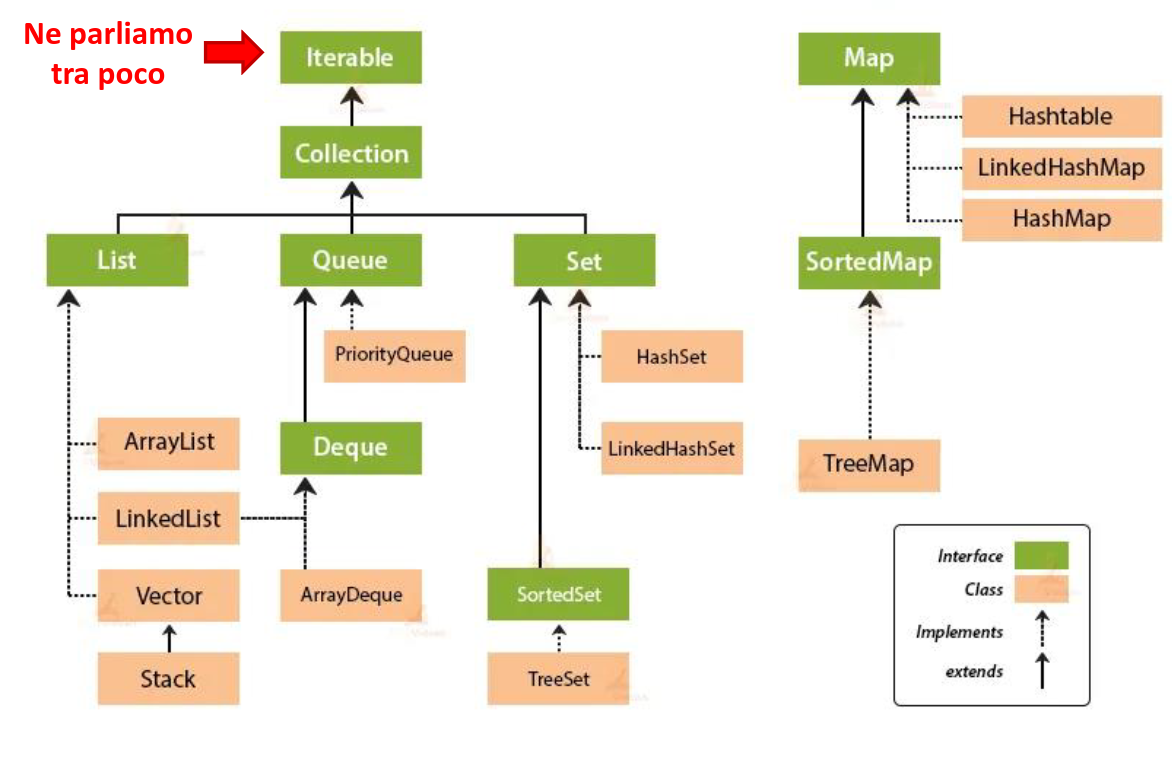
\includegraphics[width=0.98\textwidth]{jcf.png}
\end{figure}\\
Un \textbf{iteratore} è un'astrazione che permette di estrarre uno alla volta gli elementi di una collezione senza esporne la rappresentazione. Generalizza la scansione linerare di array e liste a collezioni generiche.
\begin{lstlisting}
	public interface Iterator<E> {
		boolean hasNext();
		E next();
		void remove();
	}
\end{lstlisting}
Quindi posso creare un iteratore su una certa collezione e poi usare quell'oggetto per scorrerla.\\
Il metodo \textbf{remove} esiste perché non si può rimuovere un oggetto dalla collezione mentre si sta visitando.\\
Tramite il \textbf{foreach} si può scorrere una collezione: Java sotto il cofano creerà un iteratore.